\documentclass[tikz]{standalone}
\usetikzlibrary{calc,arrows}
\usepackage{frenchmath}
\usepackage{amsmath}

\begin{document}
    \color{blue}
    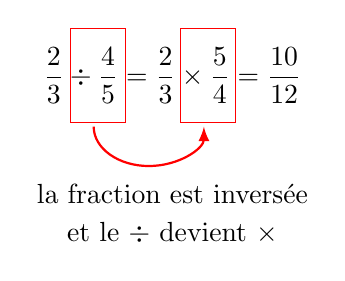
\begin{tikzpicture}
        \node at (0,0) {$\dfrac{2}{3} \div \dfrac{4}{5} = \dfrac{2}{3} \times \dfrac{5}{4} = \dfrac{10}{12}$};
        \draw[red] (0.1,-0.6) rectangle (0.8,0.6);
        \draw[red] (-1.3,-0.6) rectangle (-0.6,0.6);
        \draw[red,thick,-latex] (-1,-0.65) arc (-180:0:0.7 and 0.5);
        \node at (0,-1.5) {la fraction est inversée};
        \node at (0,-2) {et le $\div$ devient $\times$};
    \end{tikzpicture}
\end{document}